%======================================================================
\chapter{Measuring R\'{e}nyi Entanglement Entropy}
%======================================================================
\comment{Totally why do we measure this?  Y'know?}

\noindent
- we can't measure \vn with vb qmc\\
- \vb isn't a good measure of entropy\\
- can measure \re\\
 - closest entropy to \vn\\
 - gives a lower bound on \vn\\
 - maybe follows same area law and still has universal terms? (check)\\
 
The generalized Renyi entanglement entropies, again defined as:
\begin{equation}
 	S_n(\rho_{\rm A}) = \frac{1}{1-n}\ln\left[{\rm Tr}\left( \rho_{\rm A}^n \right) \right],
\end{equation}
where $\rho_{\rm{A}}=\rm{Tr}_B\ket{\psi}\bra{\psi}$ is the reduced density matrix of region A, and $n>0$.

\change{
"Encode information about the whole entanglement spectrum of $\rho_{\rm A}$."
(But that's just because if you know all of them you pretty much know all the eigenvalues of $\rho_{\rm A}$.)
So they have more information together than just $S_1=\VN$. \cite{Spectrum}
}

\change{ Something about topological entanglement entropy and quantum dimension \cite{Bbob}.}

\change{ Field theory on $O(N)$ model... universal corrections to scaling of $S_n$ calculated.}

The Renyi entropies have the property that successive entropies give a lower bound on the previous entropies.  I.e. if $n>m$ then $S_n<S_m$, so \re gives a lower bound on \vn, and \re will give the closest estimate of \vn.
%----------------------------------------------------------------------------------------------------------
\section{The Swap Operator}
%----------------------------------------------------------------------------------------------------------

\begin{figure} {
	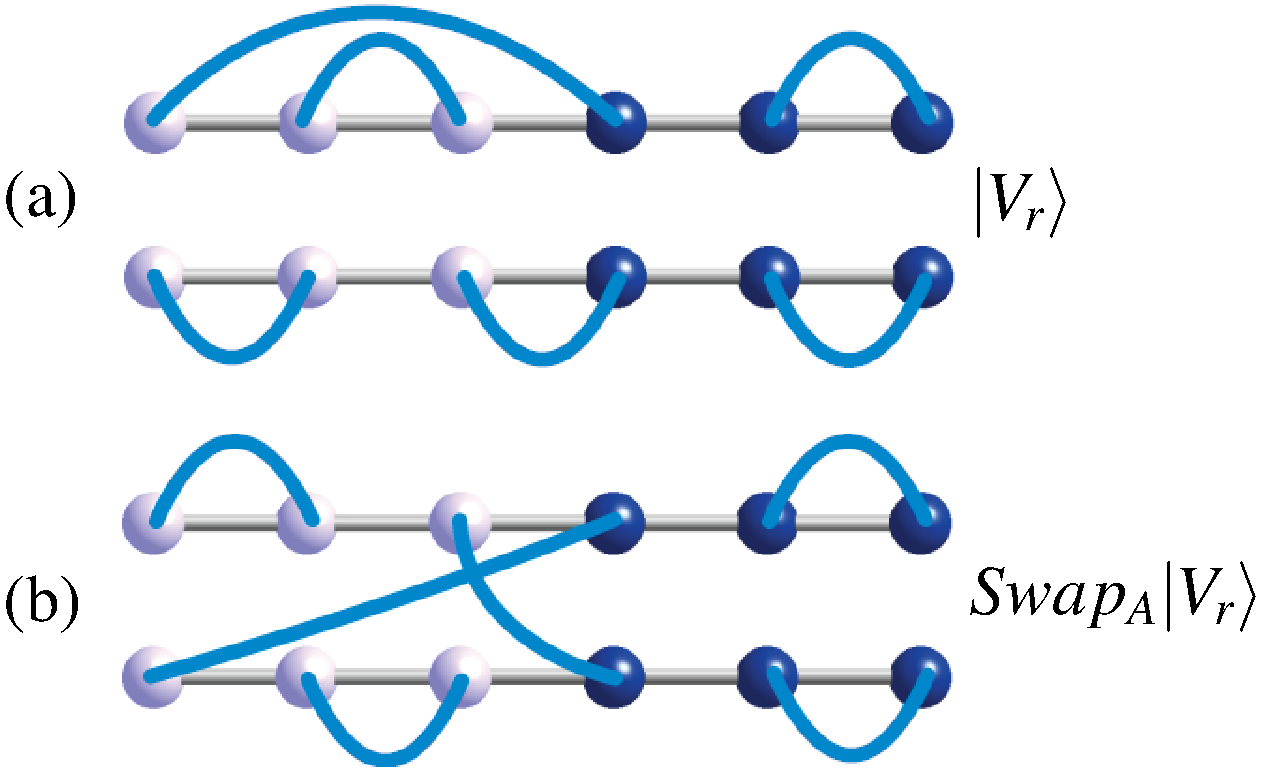
\includegraphics[width=5.5 in]{./figures/paper2/fig_swap/swap_2.pdf} 
	\centering
	\caption[Swap operator]{
	\change{Make my own, much awesomer figure.}
		\label{swap_2}
		\comment{
		A six-site chain, with two non-interacting copies (top and bottom) before
		(a) and after (b) the $Swap_A$ operation. % in the valence bond basis.  
		The region $A$ consists of three light-colored sites on the left; the
		complement region $B$ of three dark sites on the right.  The curved lines denote
		singlets in the state $|V_{r}\rangle$, which is a product of two
		different valence bond states, one per copy.
		The ground state of the entire system is a linear combination of similar $|V_{r}\rangle$.
		}
	}
}\end{figure}

%----------------------------------------------------------------------------------------------------------
\section{1D Results}
%----------------------------------------------------------------------------------------------------------

\begin{figure} {
	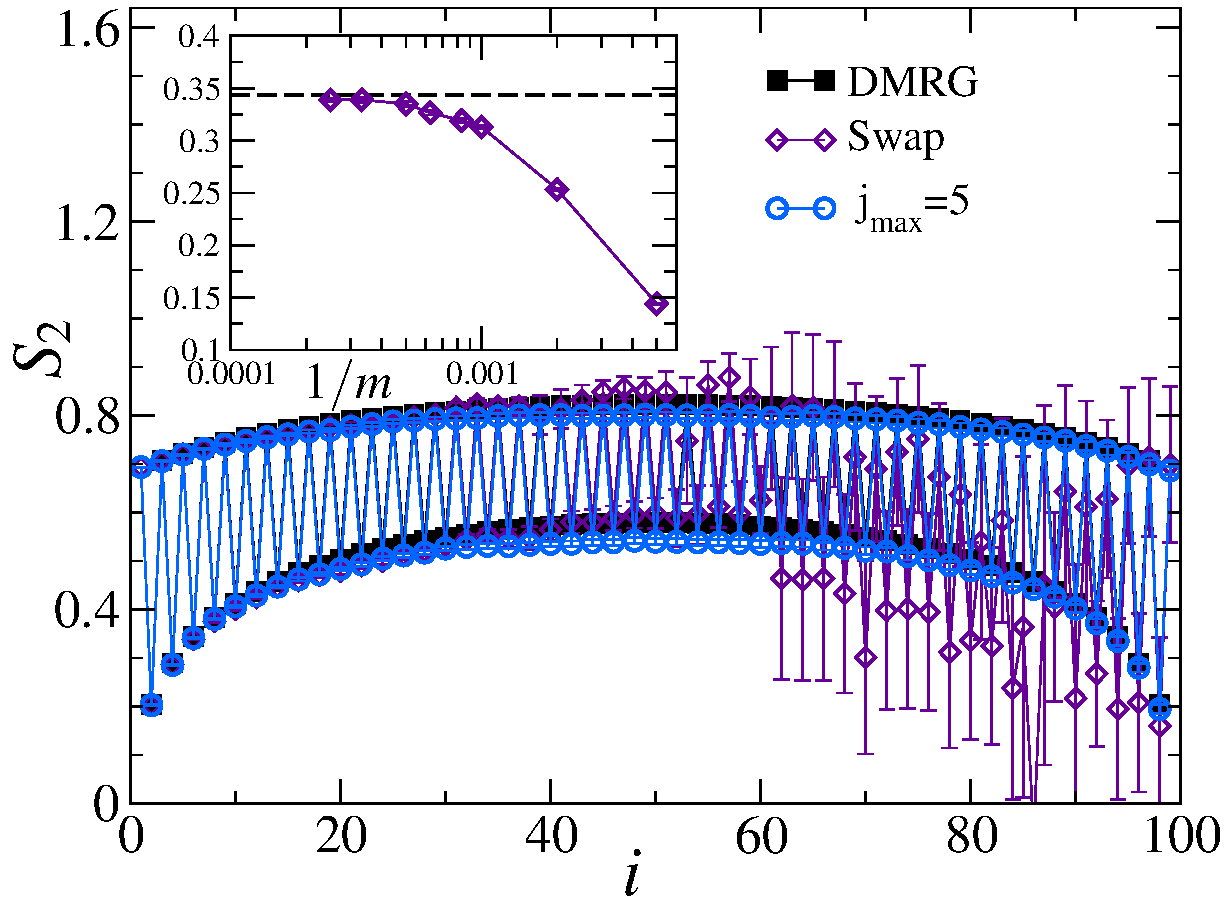
\includegraphics[width=5in]{./figures/paper2/fig_1D/L100_fig2.pdf} 
	\centering
	\caption[Renyi for 100 site chain]{ 
	\label{1Dfig}
		\comment{
		Put the Loop algorithm stuff in here?

		The Renyi entropy $S_2$ as a function of site index $i \in A$, for a 100-site Heisenberg chain with open boundaries, 
		calculated with DMRG and QMC.  Data labeled ``Swap'' was calculated with Eq.~eqref{Swap} with one QMC simulation, while
		data labeled $j_{\rm max}=5$ was calculated with Eq.~eqref{Ratio} using 20 separate QMC simulations with a range of  $j \in [1,5]$.  The inset shows the convergence of $S_2$ to the exact value (dashed line) for $i=6$ with up to $m=4000$.
		}
	}
}\end{figure}

%----------------------------------------------------------------------------------------------------------
\section{The ``Ratio Trick"}
%----------------------------------------------------------------------------------------------------------

\comment{make a diagram for this part of how the ratio stuff works.}

%----------------------------------------------------------------------------------------------------------
\section{2D Results}
%----------------------------------------------------------------------------------------------------------

\begin{figure} {
	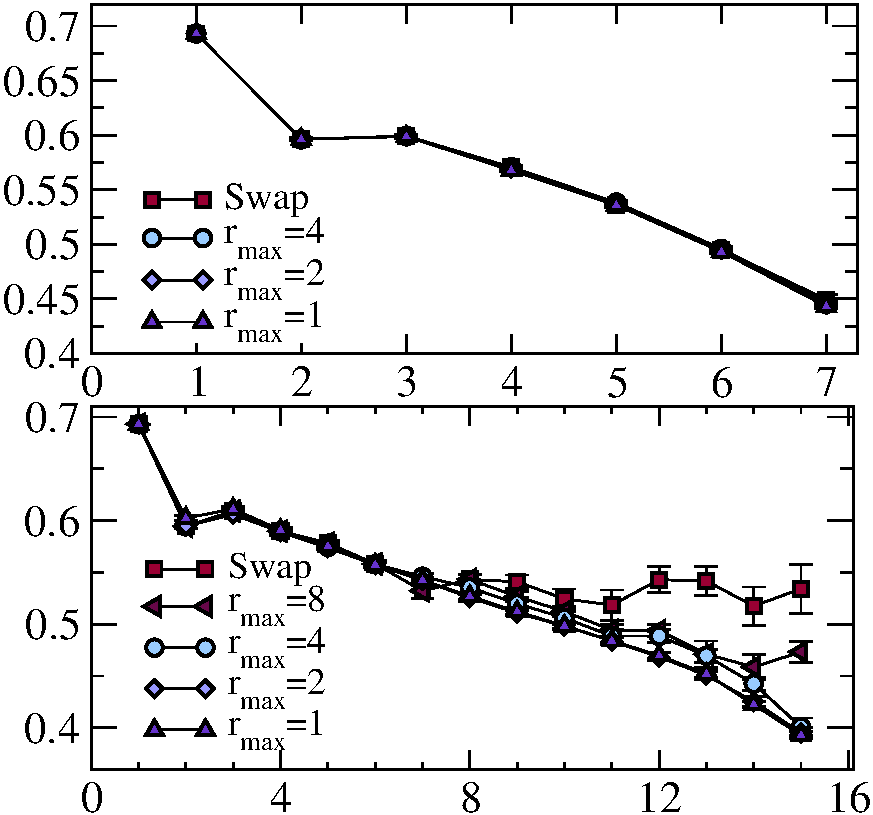
\includegraphics[width=5in]{./figures/paper2/fig_2DA/fig_L8n16.pdf} 
	\centering
	\caption[fds]{ fds
	\label{2Dfig}
	}
} \end{figure}

%----------------------------------------------------------------------------------------------------------
\section{The Area Law}
%----------------------------------------------------------------------------------------------------------

\begin{figure} {
	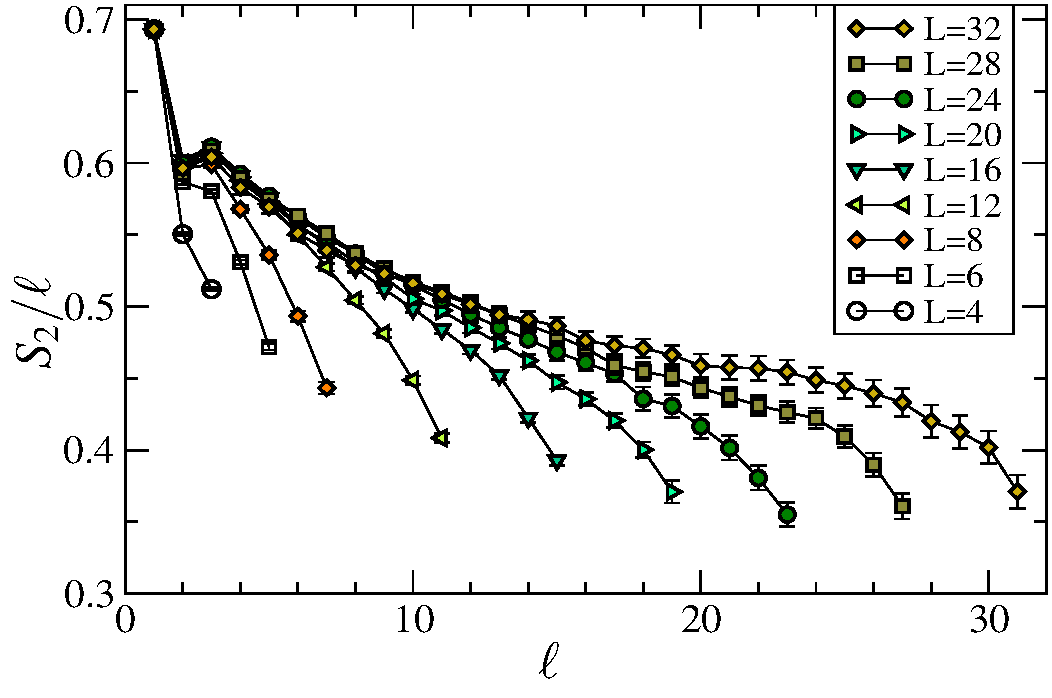
\includegraphics[width=5in]{./figures/paper2/fig_AreaL/fig4.pdf} 
	\centering
	\caption[fds]{ fds
	\label{2Dfig}
	}
} \end{figure}

\begin{figure} {
	\centering
	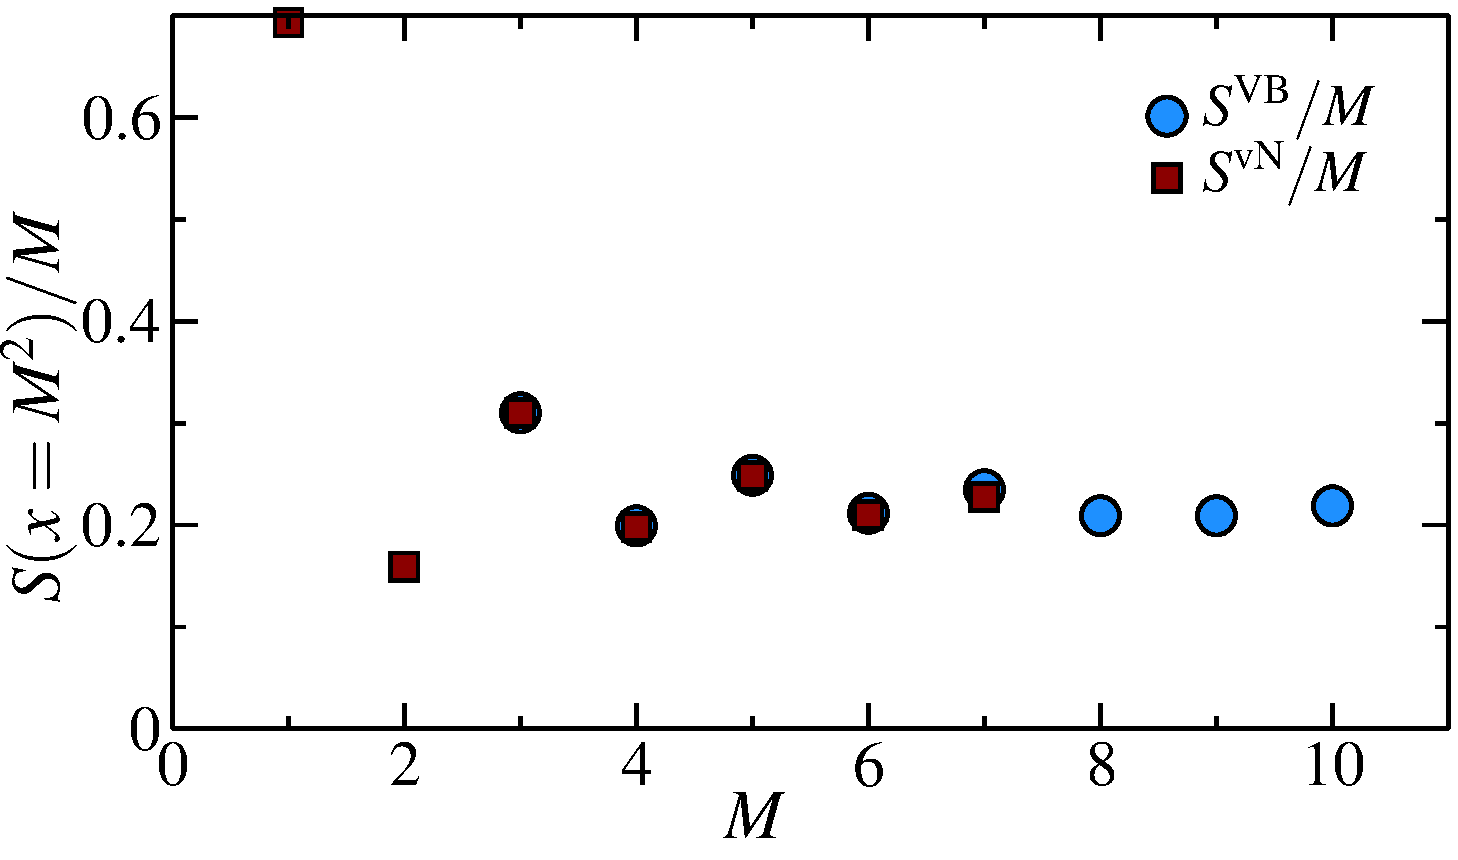
\includegraphics[width=5in]{./figures/made/marea.pdf} 
	\caption[fds]{ fds
	\label{2Dbetter}
	}
} \end{figure}
